\begin{frame}[fragile]{Design}
\vspace{-1em}
\begin{center}
	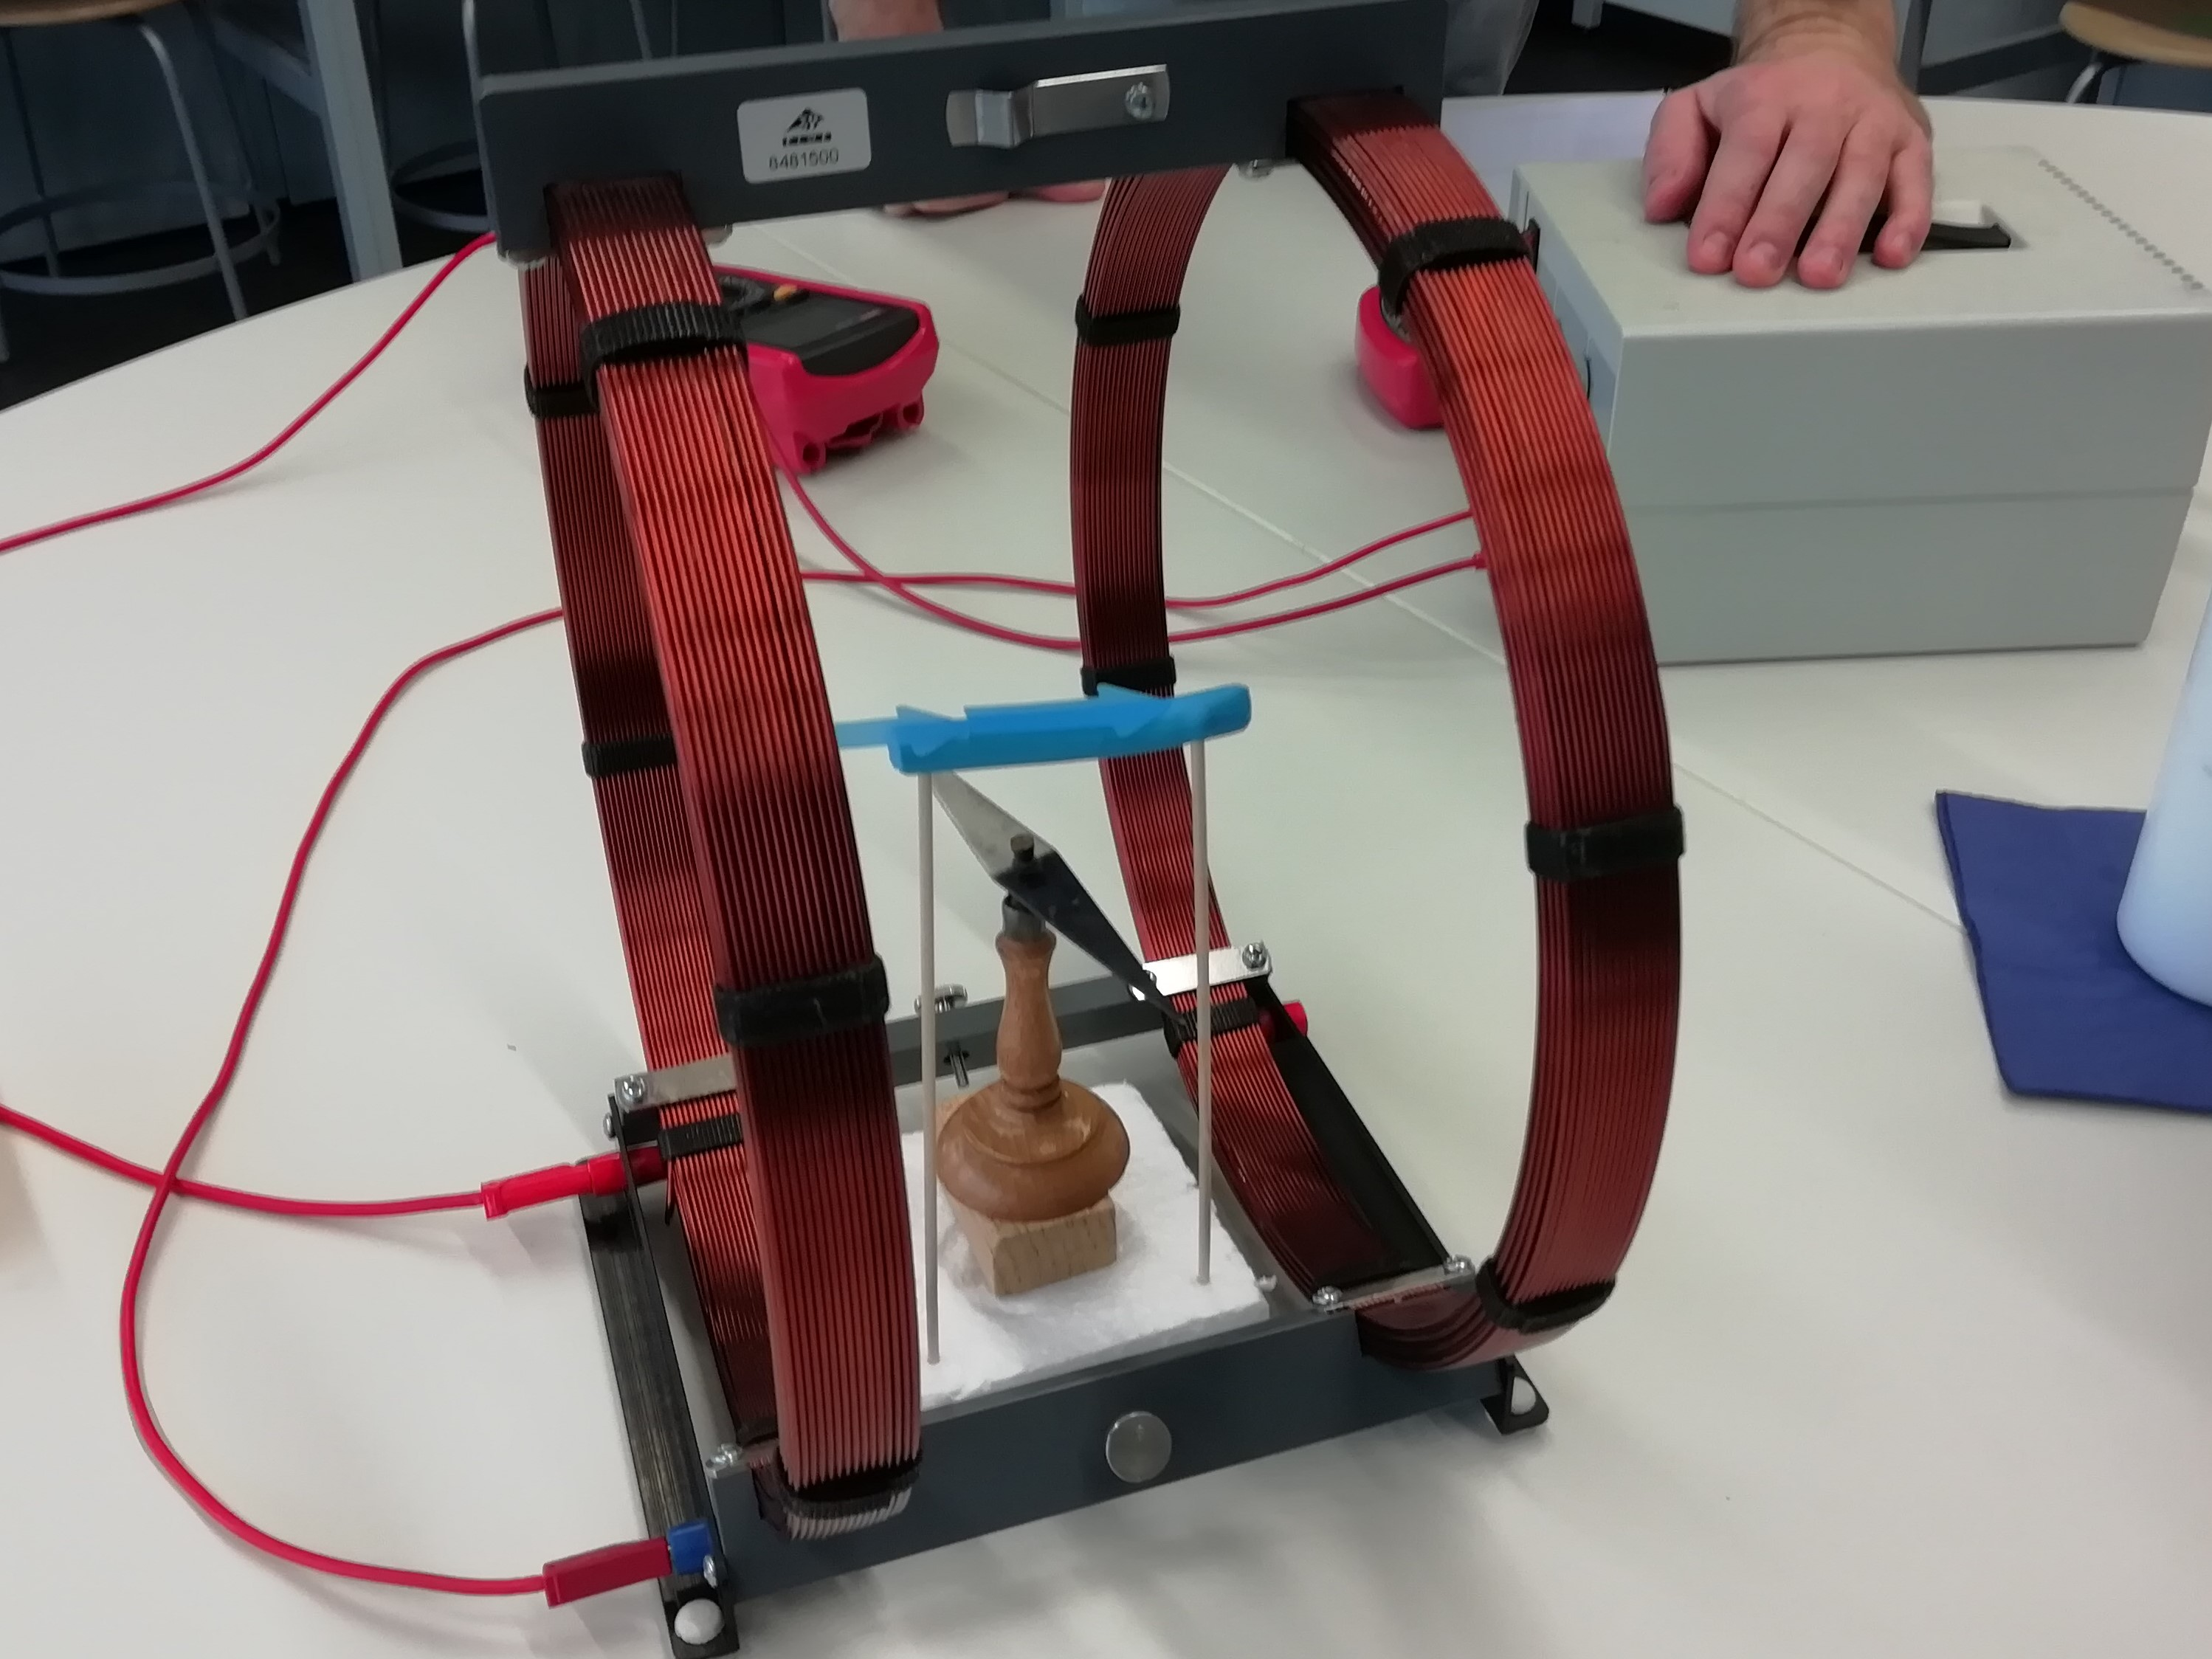
\includegraphics[width=0.33\textwidth]{images/Design_1.jpg}
	\hspace{0.05cm}
	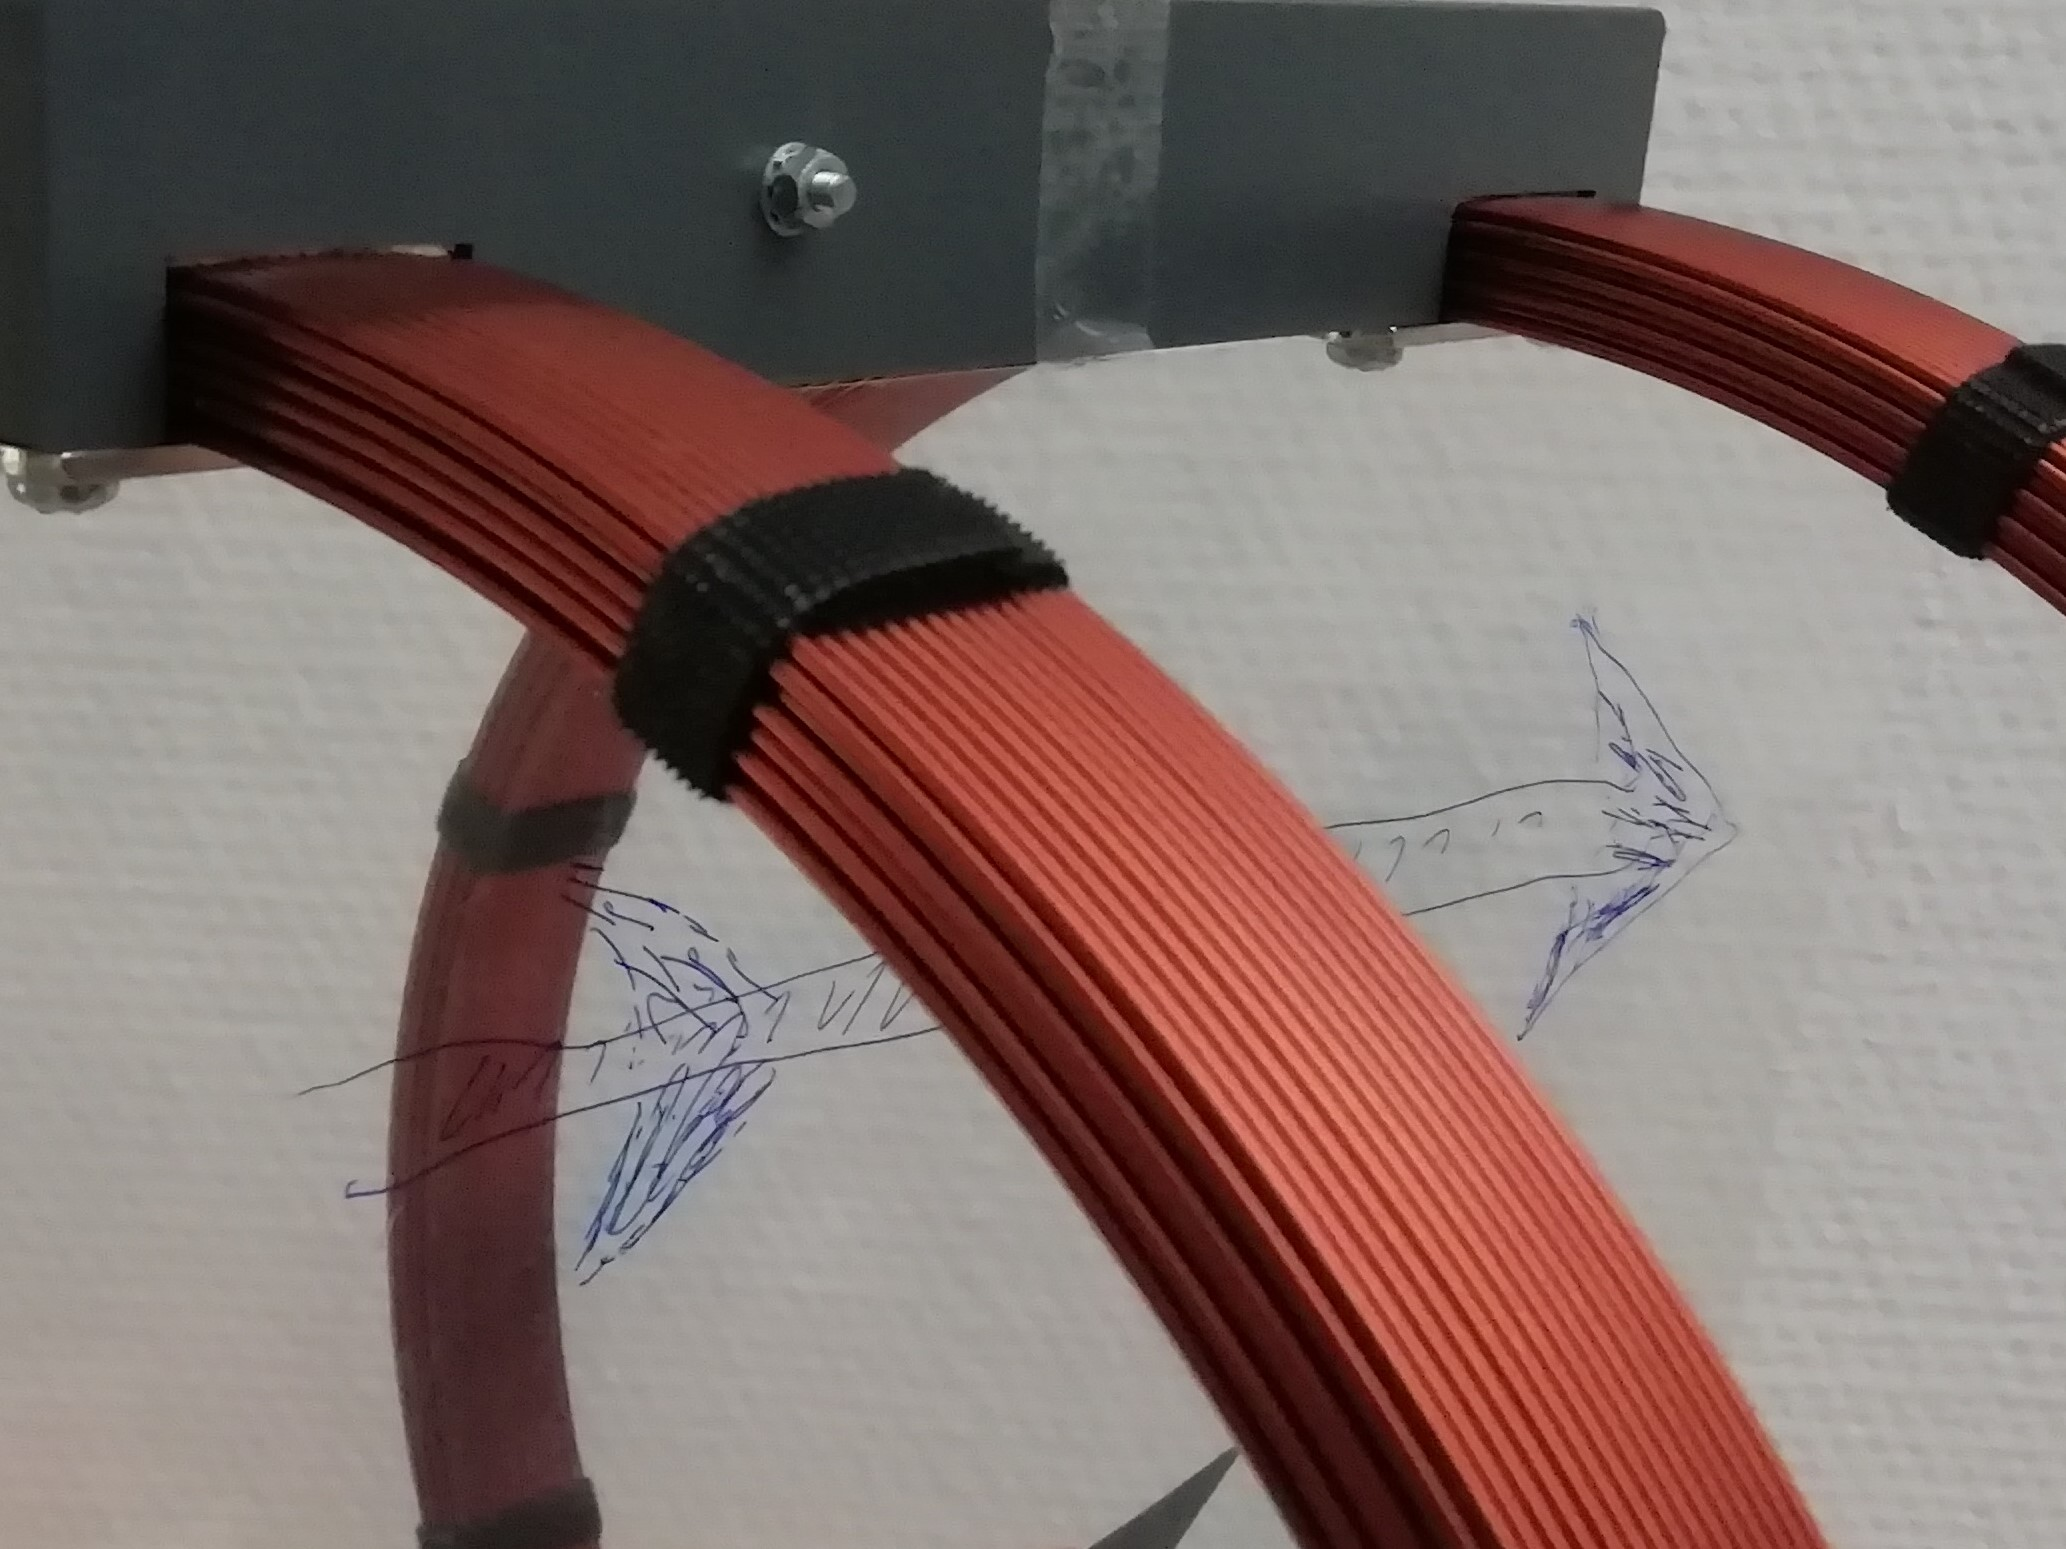
\includegraphics[width=0.33\textwidth]{images/Design_2.jpg}	
	
	
	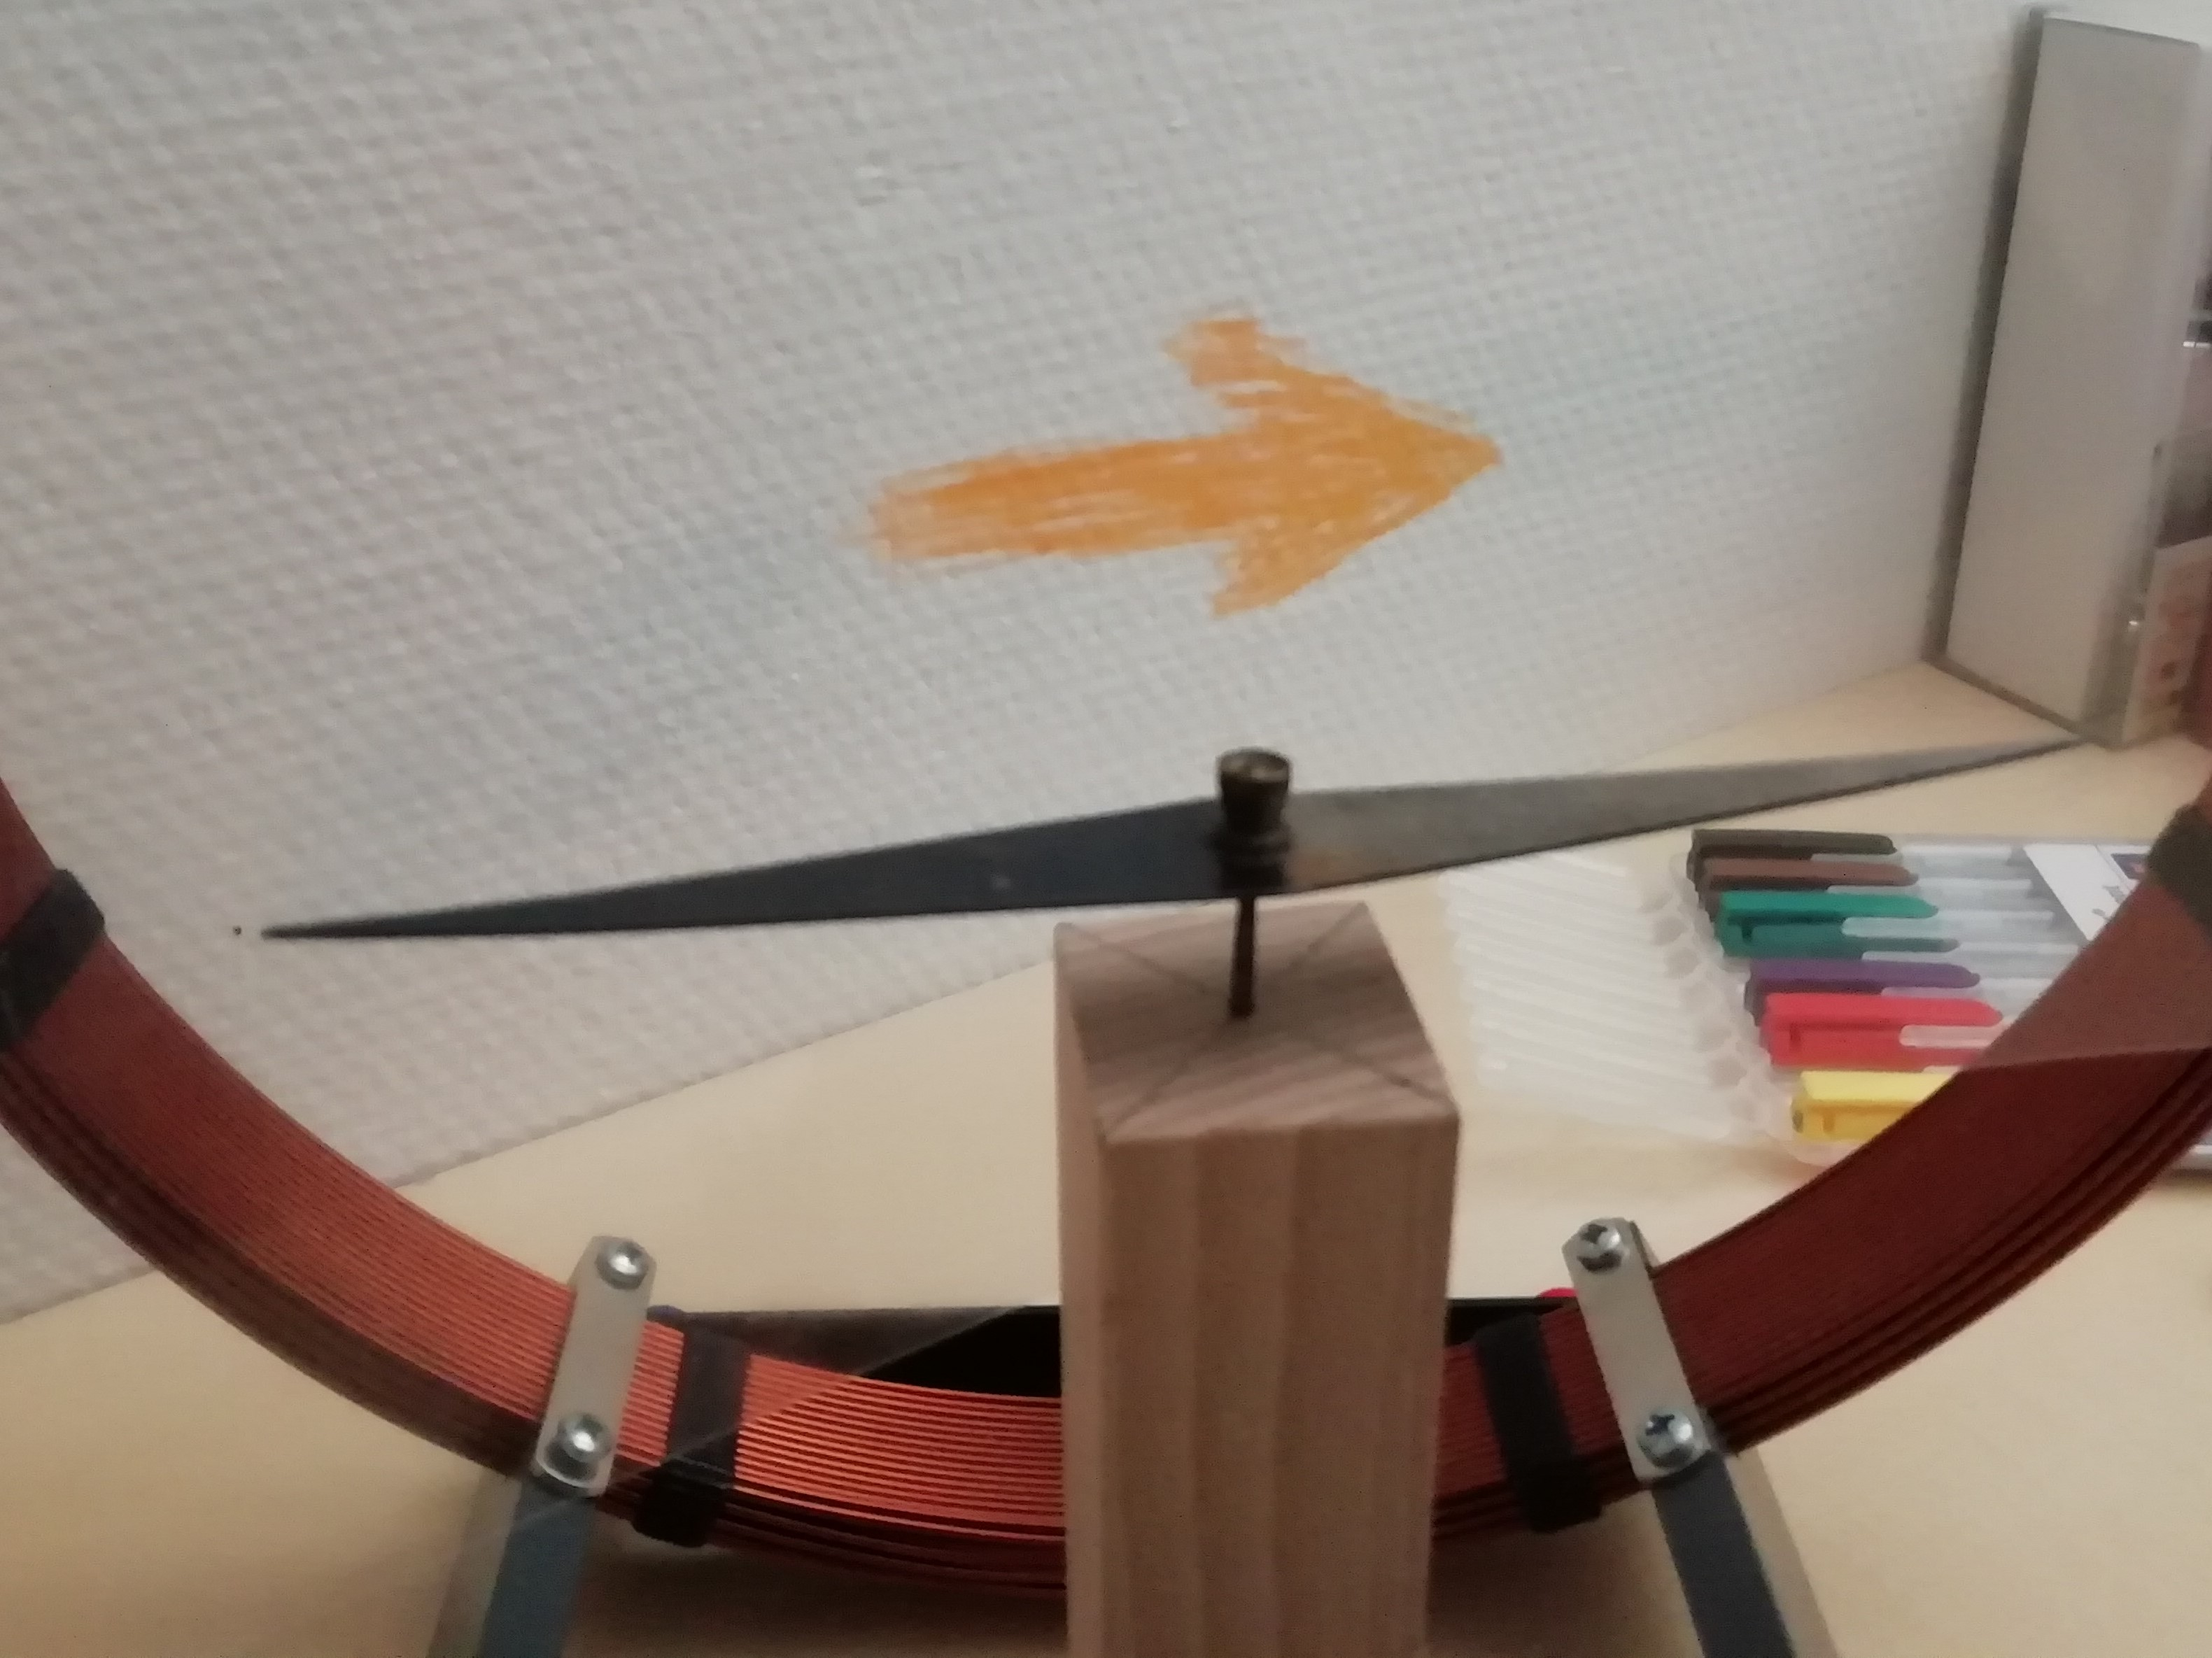
\includegraphics[width=0.33\textwidth]{images/Design_3.jpg}	
	\hspace{0.05cm}
	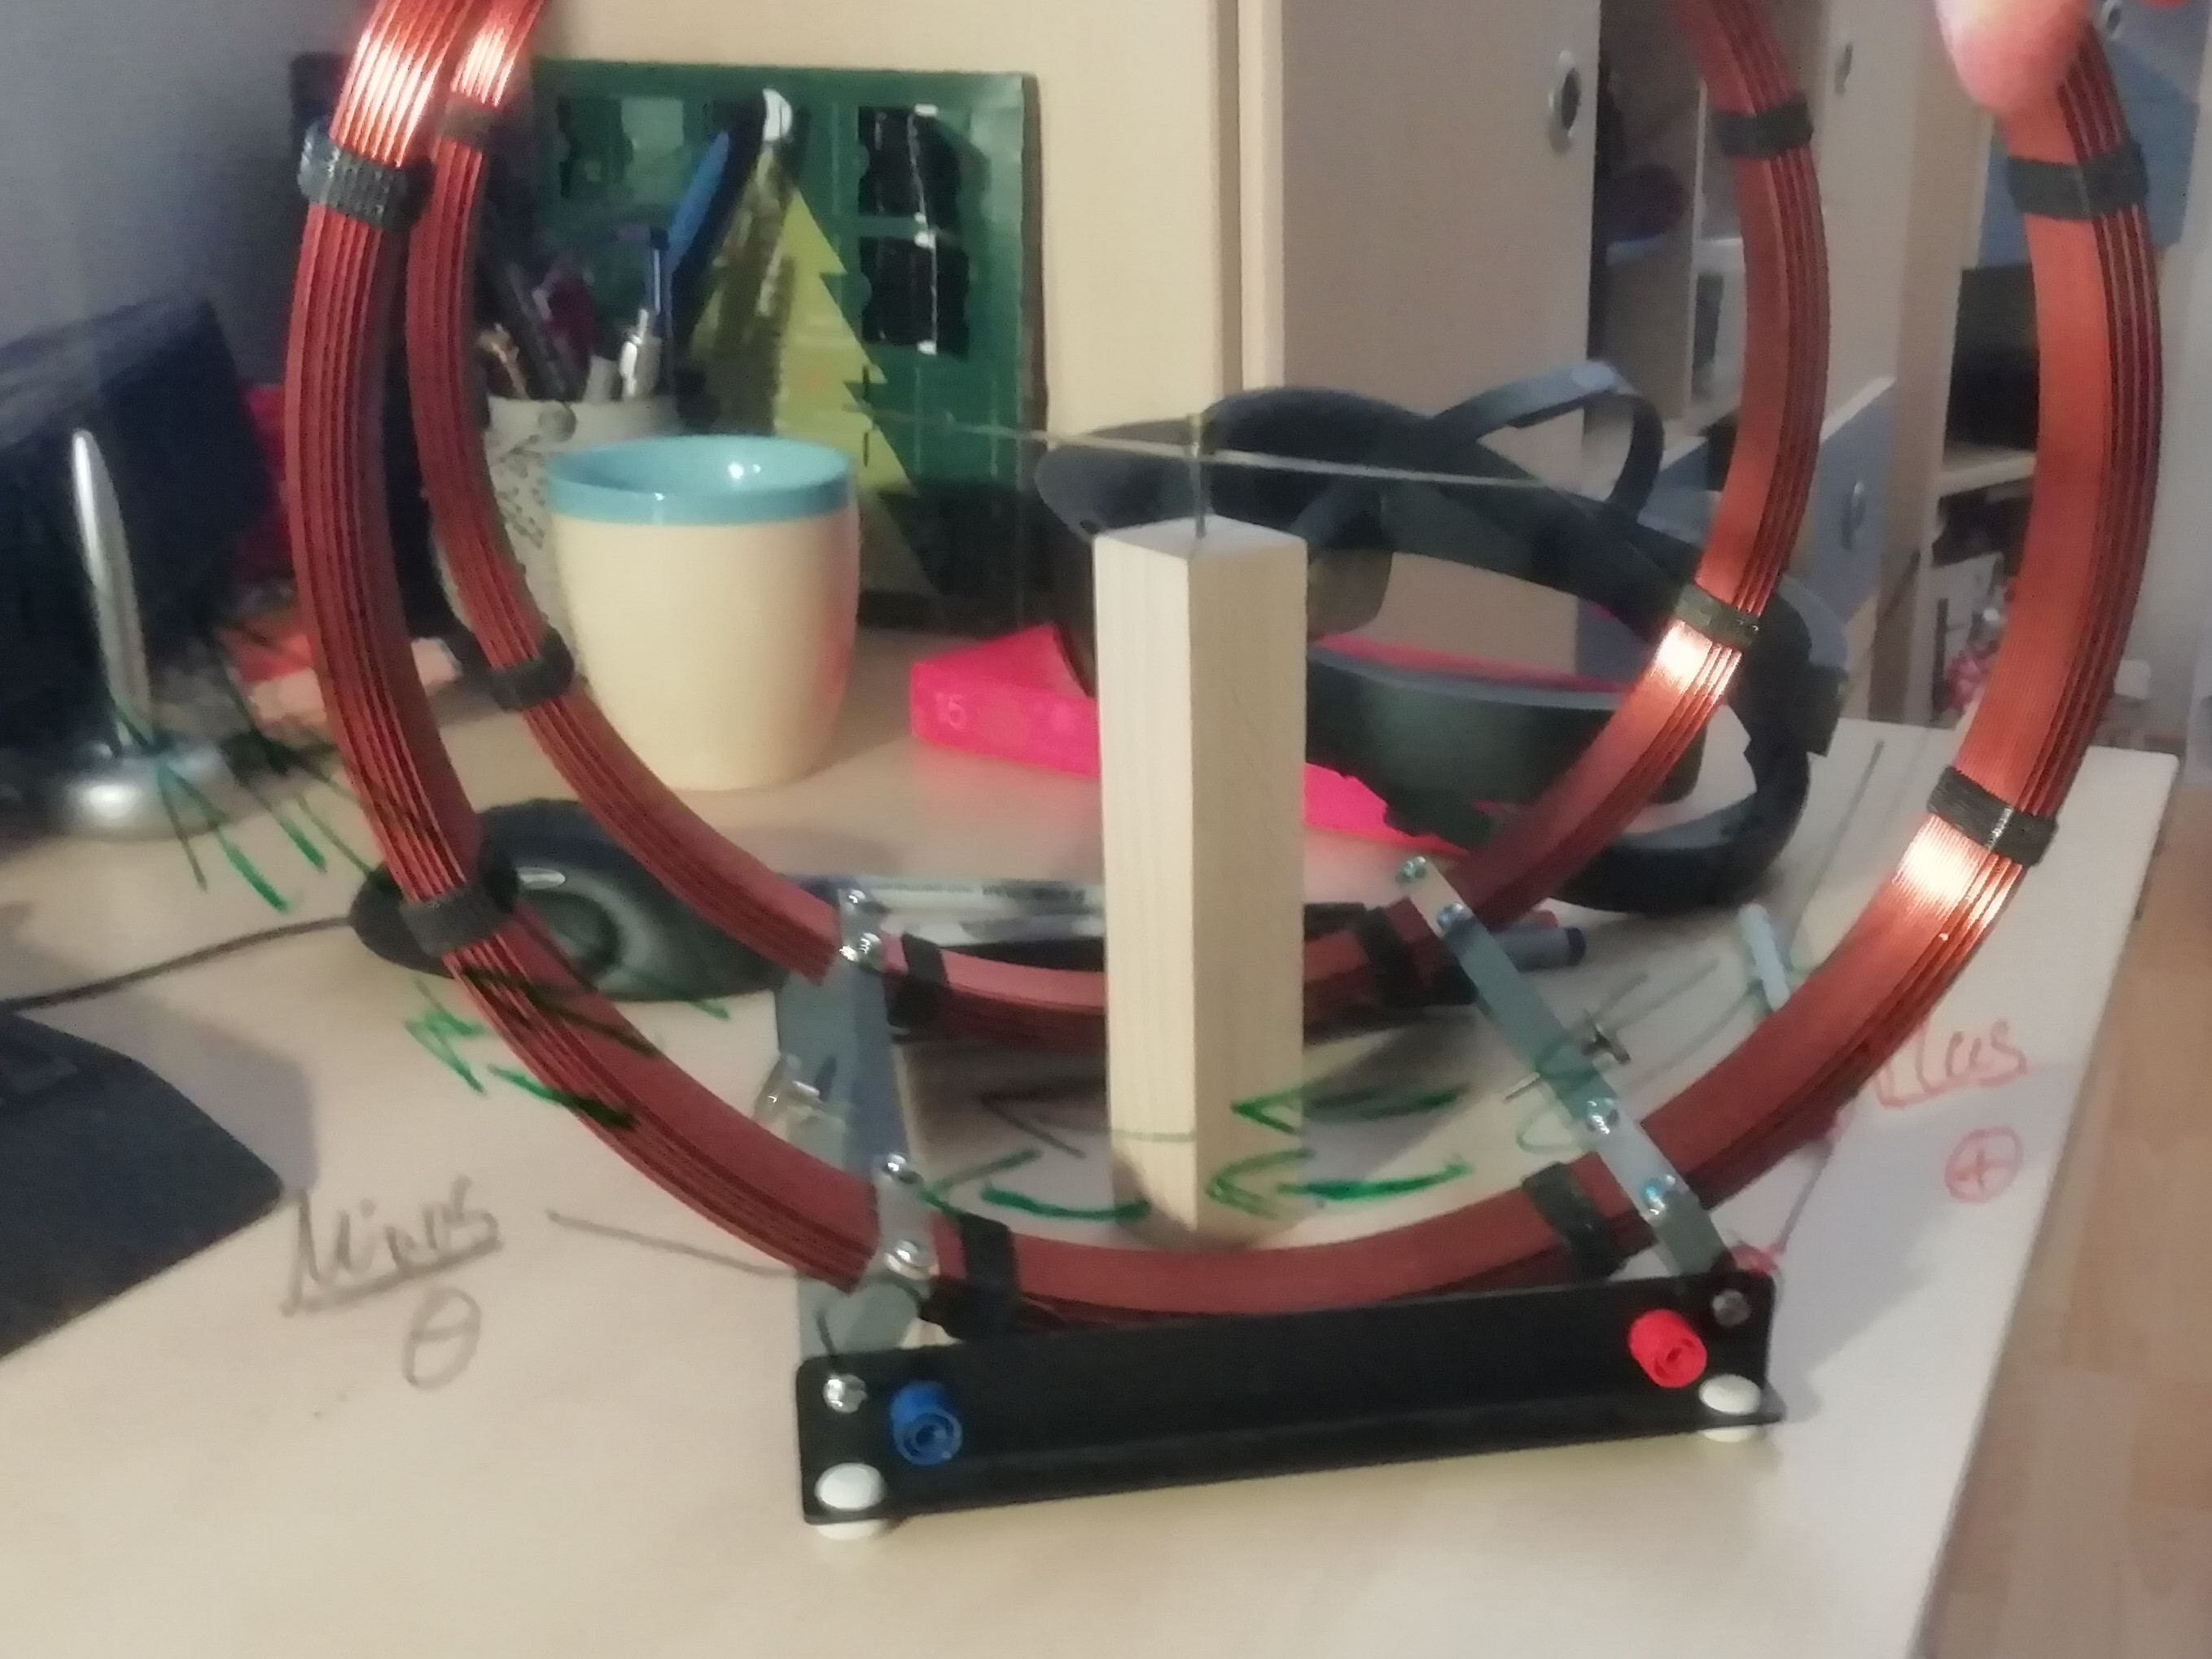
\includegraphics[width=0.33\textwidth]{images/Design_4.jpg}	
\end{center}
\end{frame}

\begin{frame}[fragile]{Field of View}
\begin{figure}
	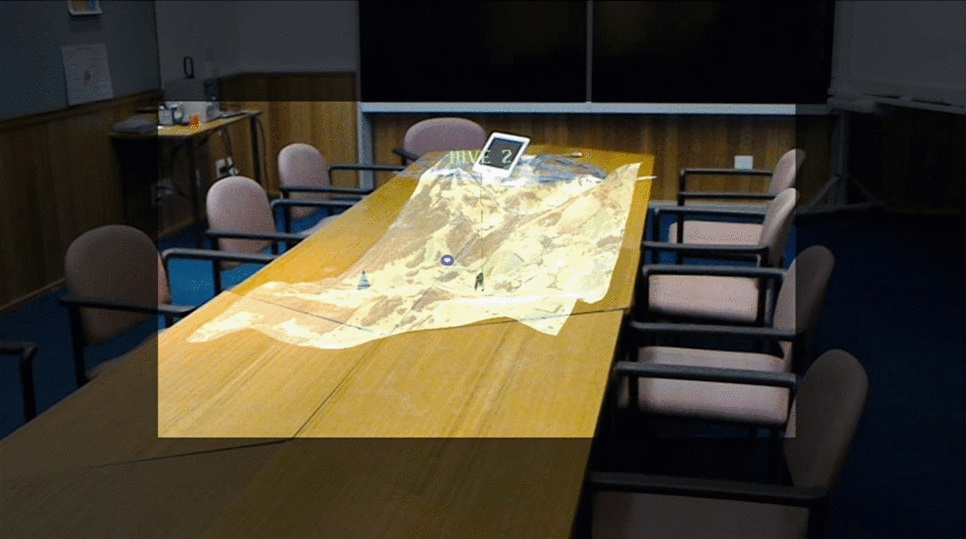
\includegraphics[width=0.8\textwidth]{images/papers/fov.jpg}\\
	\vspace{0.3cm}
	\scriptsize MRC mit hervorgehobenem, tatsächlichem FoV. Nguyen (2017).
\end{figure}
\end{frame}

\begin{frame}[fragile]{Performance}
\vspace{-1em}
\begin{center}
	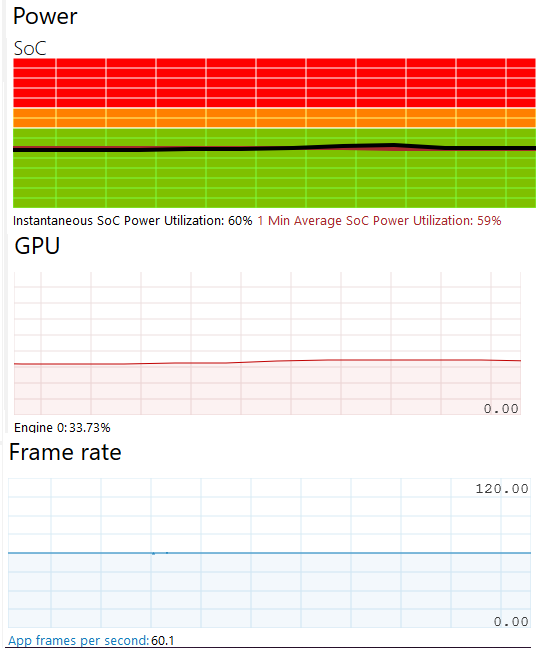
\includegraphics[width=0.4\textwidth]{images/performance/perf_msaa_off_cut.png}
	\hspace{0.05cm}
	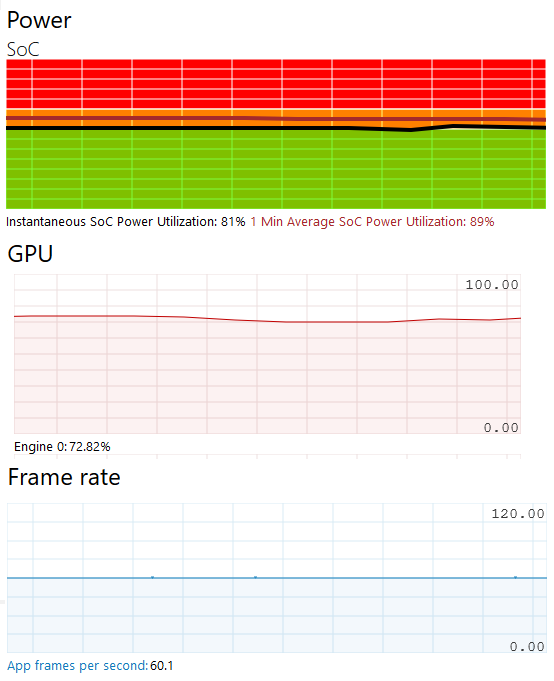
\includegraphics[width=0.4\textwidth]{images/performance/perf_msaa_on_cut.png}
\end{center}
\end{frame}

\begin{frame}[fragile]{Client-Server}
\vspace{-1em}
\begin{center}
	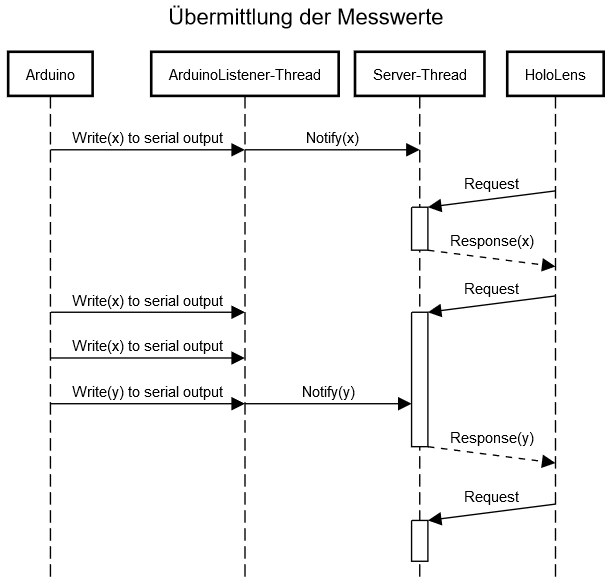
\includegraphics[width=0.6\textwidth]{images/schema/Sequenzdiagramm.png}
\end{center}
\end{frame}